\let\negmedspace\undefined
\let\negthickspace\undefined
\documentclass[journal]{IEEEtran}
\usepackage[a5paper, margin=10mm, onecolumn]{geometry}
%\usepackage{lmodern} % Ensure lmodern is loaded for pdflatex
\usepackage{tfrupee} % Include tfrupee package

\setlength{\headheight}{1cm} % Set the height of the header box
\setlength{\headsep}{0mm}     % Set the distance between the header box and the top of the text

\usepackage{gvv-book}
\usepackage{gvv}
\usepackage{cite}
\usepackage{amsmath,amssymb,amsfonts,amsthm}
\usepackage{algorithmic}
\usepackage{graphicx}
\usepackage{textcomp}
\usepackage{xcolor}
\usepackage{txfonts}
\usepackage{listings}
\usepackage{enumitem}
\usepackage{mathtools}
\usepackage{gensymb}
\usepackage{comment}
\usepackage[breaklinks=true]{hyperref}
\usepackage{tkz-euclide} 
\usepackage{listings}
% \usepackage{gvv}                                        
\def\inputGnumericTable{}                                 
\usepackage[latin1]{inputenc}                                
\usepackage{color}                                            
\usepackage{array}                                            
\usepackage{longtable}                                       
\usepackage{calc}                                             
\usepackage{multirow}                                         
\usepackage{hhline}                                           
\usepackage{ifthen}                                           
\usepackage{lscape}
\usepackage{circuitikz}
\tikzstyle{block} = [rectangle, draw, fill=blue!20, 
    text width=4em, text centered, rounded corners, minimum height=3em]
\tikzstyle{sum} = [draw, fill=blue!10, circle, minimum size=1cm, node distance=1.5cm]
\tikzstyle{input} = [coordinate]
\tikzstyle{output} = [coordinate]


\begin{document}

\bibliographystyle{IEEEtran}
\vspace{3cm}

\title{4.13.92}
\author{AI25BTECH11023-Pratik R}
 \maketitle
% \newpage
% \bigskip
{\let\newpage\relax\maketitle}

\renewcommand{\thefigure}{\theenumi}
\renewcommand{\thetable}{\theenumi}
\setlength{\intextsep}{10pt} % Space between text and floats


\numberwithin{equation}{enumi}
\numberwithin{figure}{enumi}
\renewcommand{\thetable}{\theenumi}

\subsection*{\textbf{Question}} 
The equation of a plane passing through the line of intersection of the planes $x+2y+3z=2$ and $x-y + z = 3$ and at a distance $\frac{2}{\sqrt{3}}$ from the point $(3,1,-1)$ is 
\subsection*{\textbf{Solution}}
According to the question,\\
\begin{align}
    \vec{n_1}=\myvec{1\\2\\3} \quad \vec{n_2}=\myvec{1\\-1\\1} \quad c_1=2 \quad c_2=3
\end{align}
The equation of plane which contains the line of intersection of the two planes is given by
\begin{align}
    \vec{n_1}^{\top}\vec{x}-c_1+\lambda\brak{\vec{n_2}^{\top}\vec{x}-c_2}=0
\end{align}
\begin{align}
    \implies \brak{\vec{n_1}^{\top}+\lambda\vec{n_2}^{\top}}\vec{x}=c_1+\lambda c_2
\end{align}
Let $d = \frac{2}{\sqrt{3}}$ be the distance of the plane from the point $P(3,1,-1)$ 
\begin{align}
    \therefore d = \frac{|\brak{\vec{n_1}+\lambda\vec{n_2}}^{\top}\vec{P} - \brak{c_1+\lambda c_2}|}{||\vec{n_1}+\lambda \vec{n_2}||}
\end{align}
simplifying RHS
\begin{align}
    \frac{|2\lambda|}{\sqrt{3\lambda ^2 +4\lambda +14}}
\end{align}
\begin{align}
    \therefore d^2= \frac{4\lambda ^2}{3\lambda ^2 +4\lambda +14}
\end{align}
solving this, we get
\begin{align}
   \lambda &=\frac{-7}{2} \text{ or}\\
   \lambda &= \infty
\end{align}
Hence the Equation of plane is given by
\begin{align}
    \myvec{-5&11&-1}\vec{x}=-17
\end{align}
or since $\lambda$ is $\infty$ the plane can be $\vec{n_2}^{\top} \vec{x} = 3 $ itself.
\newpage 
\begin{figure}[H]
    \centering
    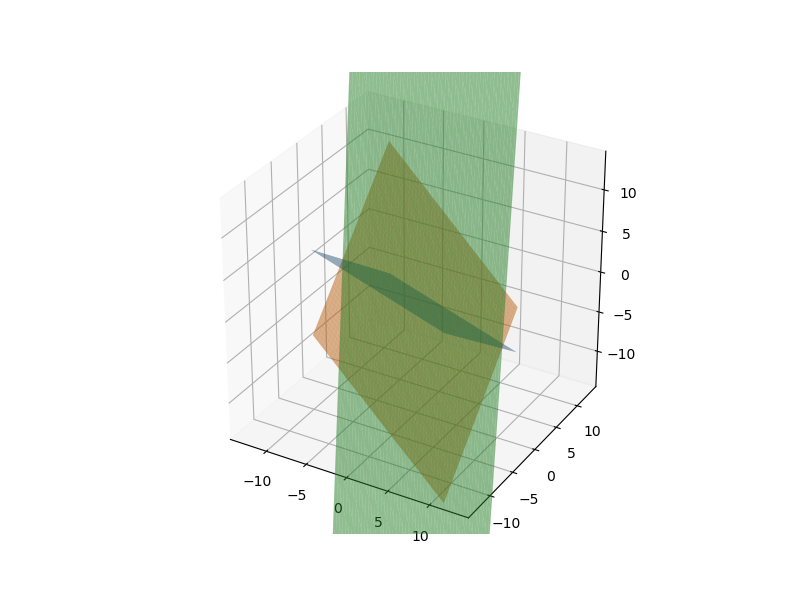
\includegraphics[width=0.8\columnwidth]{figs/fig.png}
    \label{fig:1}
\end{figure}


\end{document}